%%%%%%%%%%%%%%%%%%%%%%%%%%%%%%%%%%%%%%%%%%%%%%%%%
%------ LaTeX-Template für Abschlussarbeiten, Prof. Thomas Görne, Dezember 2012 --------
%%%%%%%%%%%%%%%%%%%%%%%%%%%%%%%%%%%%%%%%%%%%%%%%%

%---- Header (mit Formateinstellugen) laden, Inputencoding prüfen ------

%%%%%%%%%%%%%%%%%%%%%%%%%%%%%%%%%%%%%%%%%%%%%%%%%
%---- LaTeX-Header fuer Abschlussarbeiten, Prof. Thomas Goerne, Dez. 2012/Aug. 2013 ----
%%%%%%%%%%%%%%%%%%%%%%%%%%%%%%%%%%%%%%%%%%%%%%%%%

\documentclass[12pt,paper=A4,pointlessnumbers,bibtotoc,liststotoc,DIV=11,BCOR=1mm]{scrreprt}
% BCOR ist die Bindekorrektur (verlorener Rand am linken Blattrand)! Wert haengt von der Art der Heftung ab!!
% DIV ist eine Satzspiegeleinstellung von KOMA-Script / sccreprt.

\pagestyle{headings}

\usepackage[T1]{fontenc} % Font Encoding fuer europaeische Schriften mit Umlauten (Unterstuetzung der Worttrennung)
\usepackage{lmodern} % PostScript-Varianten der TeX Computer Modern-Schriften laden
\usepackage[english,ngerman]{babel} % Spracheinstellungen fuer Englisch und Neudeutsch laden

\usepackage{graphicx} % Grafikeinbindung (fuer .JPG, .JPEG, .PNG und .PDF, falls pdflatex benutzt wird)
\usepackage[table]{xcolor} % ermoeglicht farbige Schrift und farbige Tabellenzeilen
\definecolor{black}{gray}{0} % Umdefinition der Farbe black, falls noetig (0=schwarz, 1=weiss)
\definecolor{dblue}{rgb}{0.1,0.2,0.6} % Dunkelblau, fuer Hyperlinks
\definecolor{lgray}{gray}{0.9} % Hellgrau, fuer Tabellen (0=schwarz, 1=weiss)

\usepackage{booktabs} % fuer schoene Tabellen

\usepackage[round,authoryear]{natbib} % Literaturverweise mit Name/Jahreszahl in runden Klammern
\bibpunct[:\,]{(}{)}{,}{a}{}{,~}  % Feinformatierung der Natbib-Zitierweise

\usepackage[hyphens]{url}
\usepackage[colorlinks=true,linkcolor=black,citecolor=dblue,urlcolor=dblue]{hyperref} 
\usepackage{hyperref}  
% die Pakete url und hyperref ermoeglichen anklickbare URLs im Quellenverzeichnis in definierter Farbe, 
% sie ermoeglichen den Zeilenumbruch bei langen URLs, und sie erzeugen Hyperlinks (Farbe s.o.) 
% zwischen Quellenverweis und Quellenverzeichnis sowie zwischen label und ref im PDF-Dokument

% Fonteinstellungen fuer Bildunterschriften: Unterschrift serifenlos, "Abbildung" fett (bfseries = bold face series)
\setkomafont{captionlabel}{\sffamily\bfseries}
\setkomafont{caption}{\sffamily}

%------------------------------------------------------------------------------------------------------------------
%------ Eigenstaendigkeitserklaerung im gerahmten Kasten (parbox in einer framebox) ------
%------------------------------------------------------------------------------------------------------------------

\newcommand{\eigen}{
\setlength{\fboxsep}{2ex}
\setlength{\fboxrule}{0.8pt} 
% Einstellungen fuer Rahmenabstand und Rahmendicke der Framebox
\begin{center}
	\fbox{
		\parbox{0.8\linewidth}{
		Ich versichere, die vorliegende Arbeit selbstst\"andig ohne fremde Hilfe verfasst 
		und keine anderen Quellen und Hilfsmittel als die angegebenen benutzt zu haben. 
		Die aus anderen Werken w\"ortlich entnommenen Stellen oder dem Sinn nach 
		entlehnten Passagen sind durch Quellenangaben eindeutig kenntlich gemacht.
		\par\bigskip\bigskip\bigskip\bigskip
		\hspace*{0.8cm}Ort, Datum \hfill \vorname~\nachname\hspace*{0.8cm}
		}
	}
\end{center}
}

%%%%%%%%%%%%%%%%%%%%%%%%%%%%%%%%%%%%%%%%%%%%%%%%%


%------------------------ Titelblatt-Layout laden ----------------------------------

%%%%%%%%%%%%%%%%%%%%%%%%%%%%%%%%%%%%%%%%%%%%%%%%%
%------ LaTeX-Titelblatt fuer Bachelorarbeiten, Prof. Thomas Goerne, Dezember 2012 -------
%------------------------------------------------------------------------------------------------------------------
%--------------------------------- Deklarationen fuer die Titelseite  --------------------------------------
%%%%%%%%%%%%%%%%%%%%%%%%%%%%%%%%%%%%%%%%%%%%%%%%%

\title{\titel\\[2ex]
\LARGE Bachelor-Thesis\\
\large zur Erlangung des akademischen Grades B.Sc.\\[1.5ex]
\LARGE \vorname~\nachname\\[0.5ex] 
\large \matrikelnummer
}

\author{\unitlength1mm
\large\raisebox{-1ex}{
\includegraphics[width=4em]{HAW_wuerfel}}\hspace{1ex}
\parbox[b]{11.2cm}{\sffamily\large%
Hochschule f\"ur Angewandte Wissenschaften Hamburg\\[-0.2ex]
Fakult\"at Design, Medien und Information\\[-0.2ex]
Department Medientechnik
}\\[6ex]
\sffamily\large Erstpr\"ufer: \erstpruef\\[0.5ex]
\sffamily\large Zweitpr\"ufer: \zweitpruef}

%%%%%%%%%%%%%%%%%%%%%%%%%%%%%%%%%%%%%%%%%%%%%%%%%
%\input{hawmt-master-titelblatt}

%---------------------------- Titeldefinitionen --------------------------------------

\newcommand{\vorname}{Matthias}
\newcommand{\nachname}{Held}
\newcommand{\matrikelnummer}{2182712}

\newcommand{\titel}{"Red Tail":\\ Auswirkung eines zusätzlichen tiefroten Spektralanteils auf das Weißlicht von LED-Scheinwerfern \\[0.2ex] 
				\Large - am Beispiel der Beleuchtung von Hauttönen im TV-Bereich}

\newcommand{\erstpruef}{Prof. Dr. Roland Greule}
\newcommand{\zweitpruef}{Matthias Allhoff}

\date{vorläufige Fassung vom \today}   % praktisch für Vorab-Versionen. 
%\date{\sffamily Hamburg, 2. 2. 2020}  % Abgabedatum!

%--------------------------------------------------------------------------------------
%----------------------------- hier gehts los! --------------------------------------
%--------------------------------------------------------------------------------------

\begin{document}
\selectlanguage{ngerman}
\maketitle           % Titelseite erzeugen
\tableofcontents % Inhaltsverzeichnis erzeugen
\clearpage          % Seitenumbruch


%------------ Zusammenfassung / Abstract ------------------

\thispagestyle{empty}
\selectlanguage{english}
\section*{\centering\abstractname}
Form and layout of this \LaTeX-template incorporate the guidelines for theses in the Media Technology Department \glqq Richtlinien zur Erstellung schriftlicher Arbeiten, vorrangig Bachelor-Thesis (BA) und Master-Thesis (MA) im Department Medientechnik in der Fa\-kul\-t{\"a}t DMI an der HAW Hamburg\grqq\ in the version of December 6, 2012 by Prof.\ Wolfgang Willaschek. 

The thesis should be printed single-sided (simplex). The binding correction (loss at the left aper edge due to binding) might be adjusted, according to the type of binding. This template incorporates a binding correction as BCOR=1mm (suitable for adhesive binding) in the \LaTeX\ document header.

{\bfseries This is the english version of the opening abstract} (don't forget to set \LaTeX's language setting back to ngerman after the english text). 
 
 
\selectlanguage{ngerman}
\section*{\centering\abstractname}
Diese \LaTeX-Vorlage ber{\"u}cksichtigt in Form und Layout die Vorgaben f{\"u}r Abschlussarbeiten im Department Medientechnik \glqq Richtlinien zur Erstellung schriftlicher Arbeiten, vorrangig Bachelor-Thesis (BA) und Master-Thesis (MA) im Department Medientechnik in der Fakult{\"a}t DMI an der HAW Hamburg\grqq, Fassung vom 6. Dezember 2012 von Prof. Wolfgang Willaschek.
 
Der Ausdruck soll einseitig erfolgen (Simplex). Je nach Bindung ist ggf. die Bindekorrektur (Verlust am linken Seitenrand durch die Bindung) noch anzupassen. In dieser Vorlage ist eine Bindekorrektur im header der \LaTeX-Datei mit BCOR=1mm f{\"u}r Klebebindung eingestellt.

{\bfseries Das ist die deutsche Version der vorangestellten Zusammenfassung. Beide Versionen -- englisch und deutsch -- sind verbindlich!}


%--------------------------- Text -------------------------------

\chapter{Ein Kapitel}

\section{Unterkapitel mit Mathematik, Bildern und Querverweisen}

Bilder werden in \LaTeX\ am einfachsten mit includegraphics eingebunden und in eine figure-Umgebung eingebettet. Sie können mit optionalen Parametern skaliert werden; in Abbildung \ref{b_trommelmik} ist die Bildbreite auf das 0.8-fache des Satzspiegels skaliert.

Zu jeder Abbildung gehört eine nummerierte Bildunterschrift und ein Verweis im Text (Abb. \ref{b_trommelmik}). \LaTeX\ unterstützt das mit dem caption-Befehl. Mit den Befehlen label und ref werden symbolische Labels definiert und abgerufen. Für Seitenverweise wird der Befehl pageref genutzt: Richtcharakteristiken sind i.Allg. frequenzabhängig (Abb. \ref{b_richtch} auf S. \pageref{b_richtch}). 

Mit label und ref kann man nicht nur auf Bilder oder Tabellen verweisen, sondern auf jede nummerierte Struktur, z.B. auf Gleichungen, Kapitel oder Unterkapitel: Zu Fußnoten siehe Abschnitt \ref{sec_fussnot}. 

%----------- BILD ANFANG -------------
\begin{figure}[htp]     % h=here, t=top, b=bottom, p=page
\centering
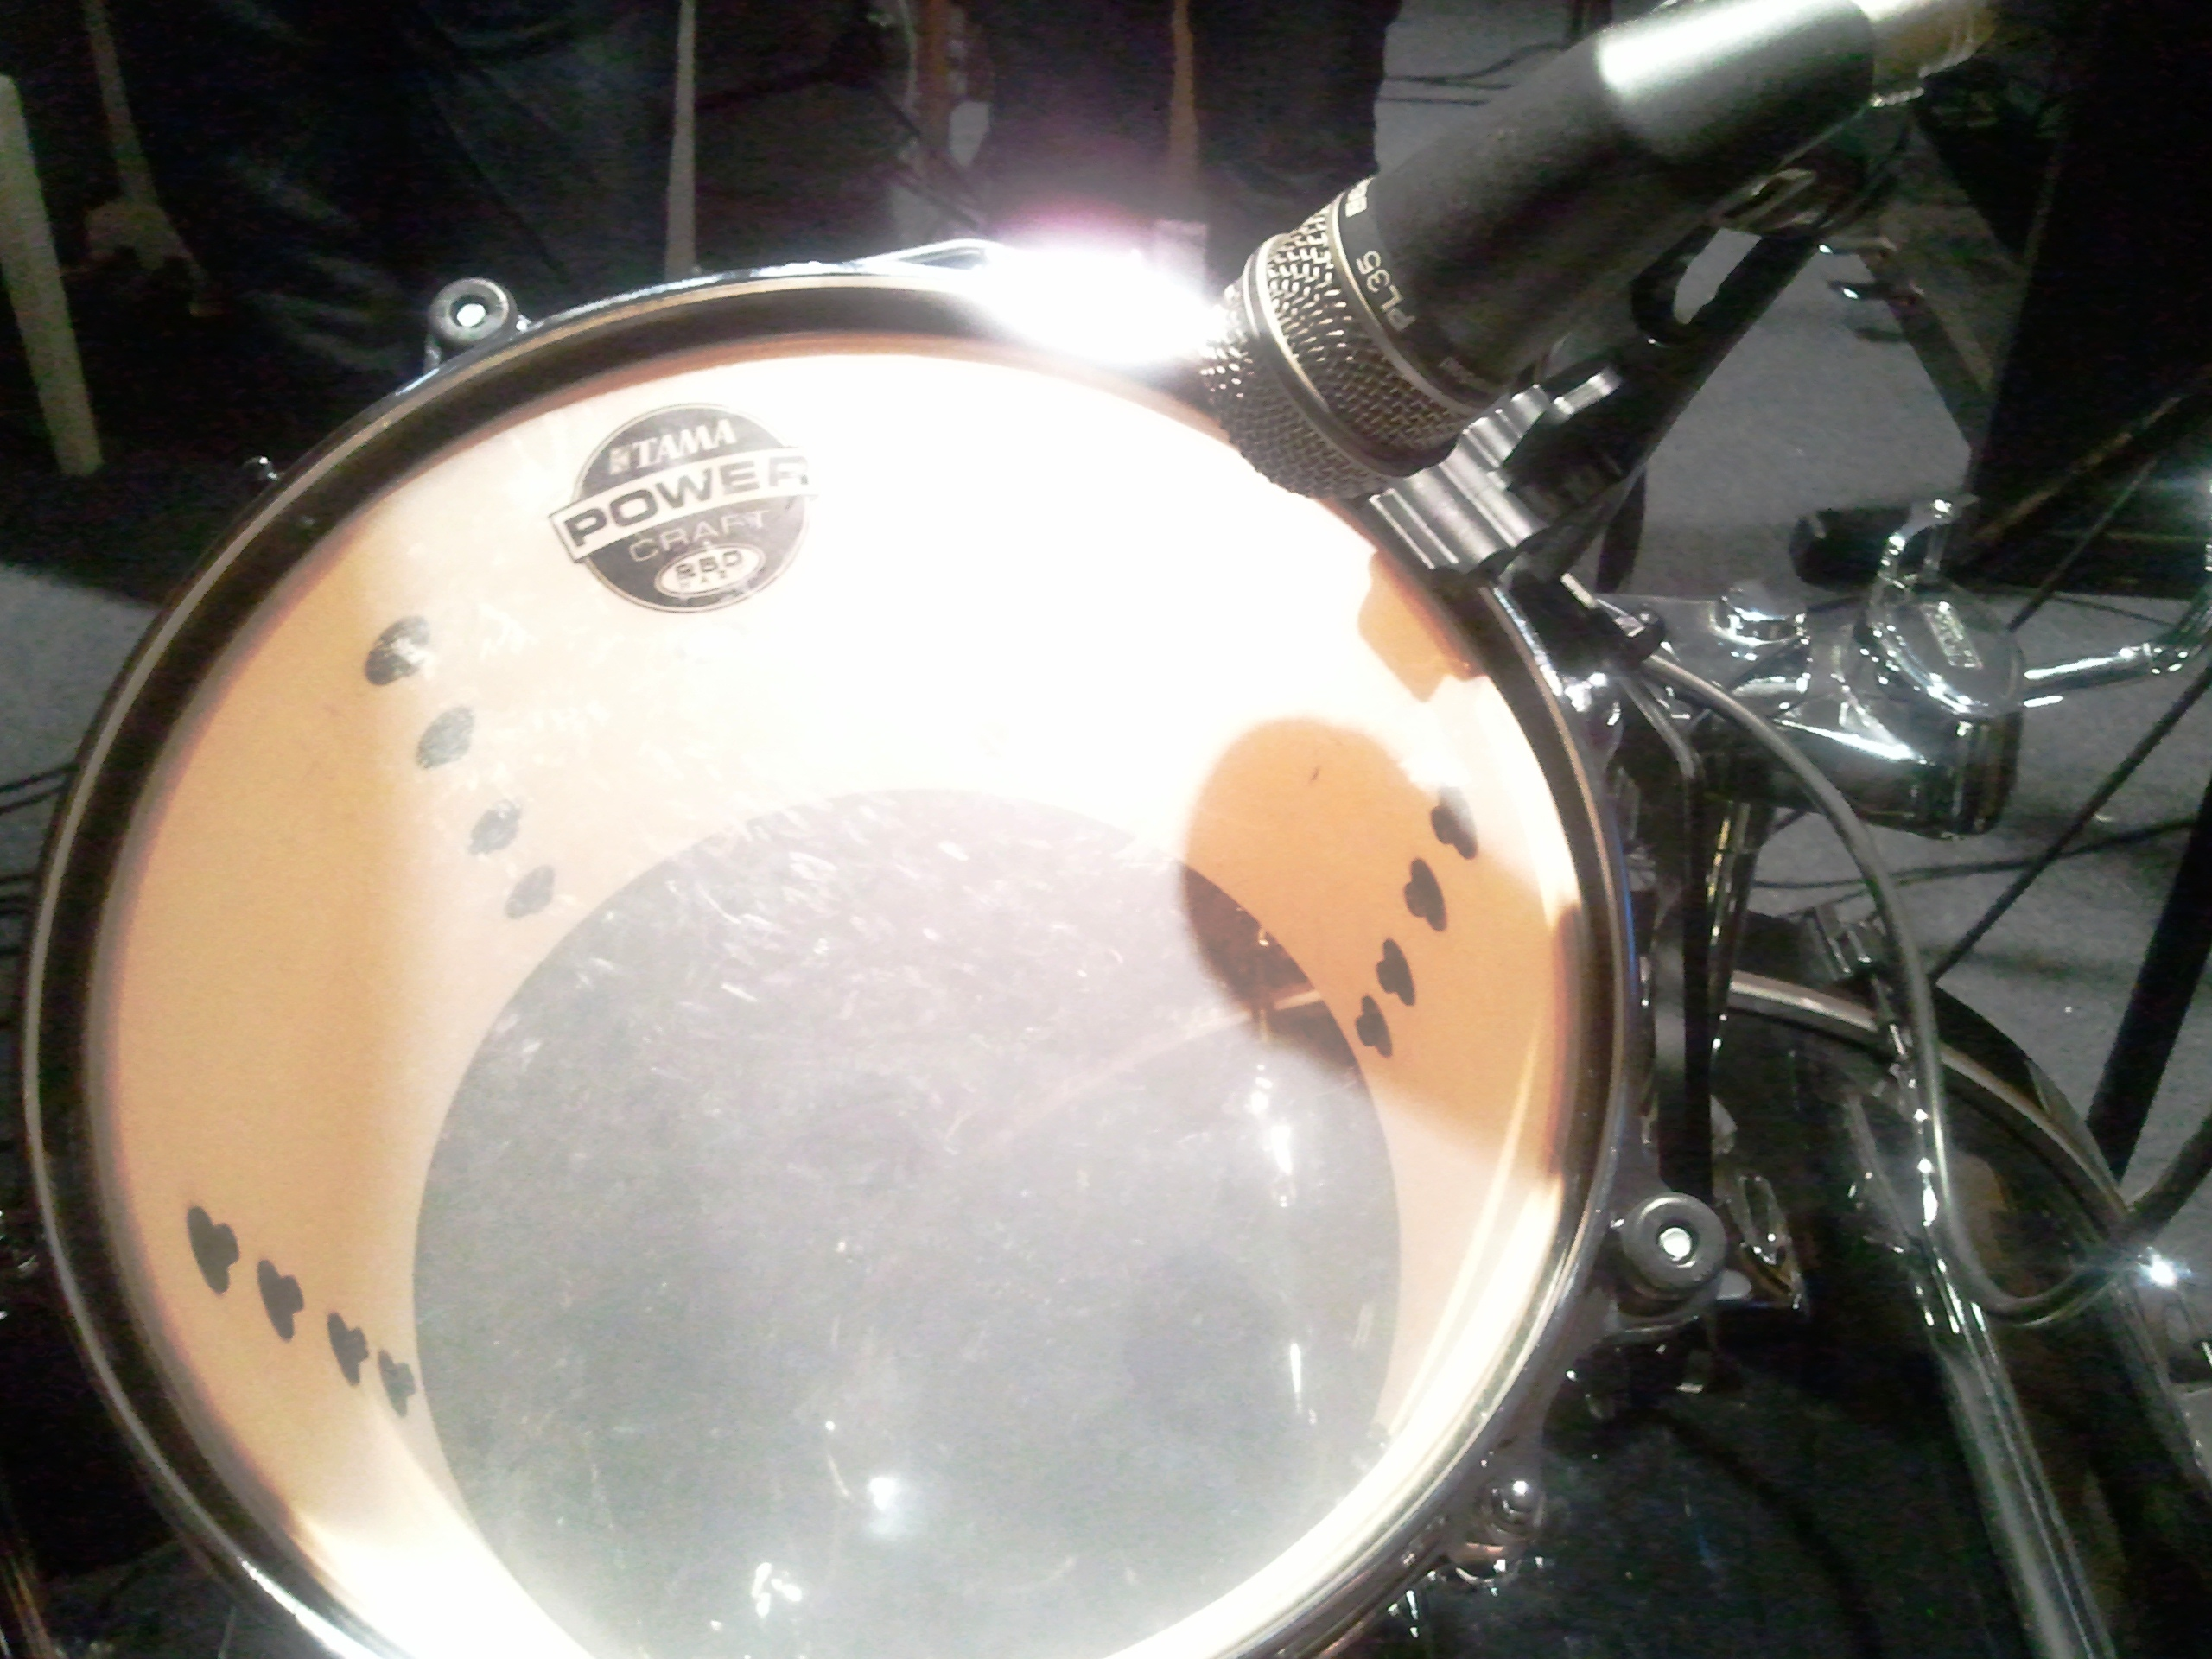
\includegraphics[width=0.8\textwidth]{bilder/drums} 
% Bilddatei aus dem Unterverzeichnis bilder holen, skalieren auf 0.8*Satzspiegel
\caption{Abnahme einer Trommel mit speziellem Anklemm-Mikrofon}\label{b_trommelmik}
\end{figure}
%------------- BILD ENDE ---------------

Praktische Tipps für die Erstellung von Bildern: Auflösung 300 dpi, bei Fotos genügen u.U. 150 dpi. Bei Scans von Strichzeichnungen sollte die Auflösung bezogen auf die Druckgröße mindestens 1200 dpi betragen (siehe Abb. \ref{b_richtch}). 

%----------- BILD ANFANG -------------
\begin{figure}[htp]     % h=here, t=top, b=bottom, p=page
\centering
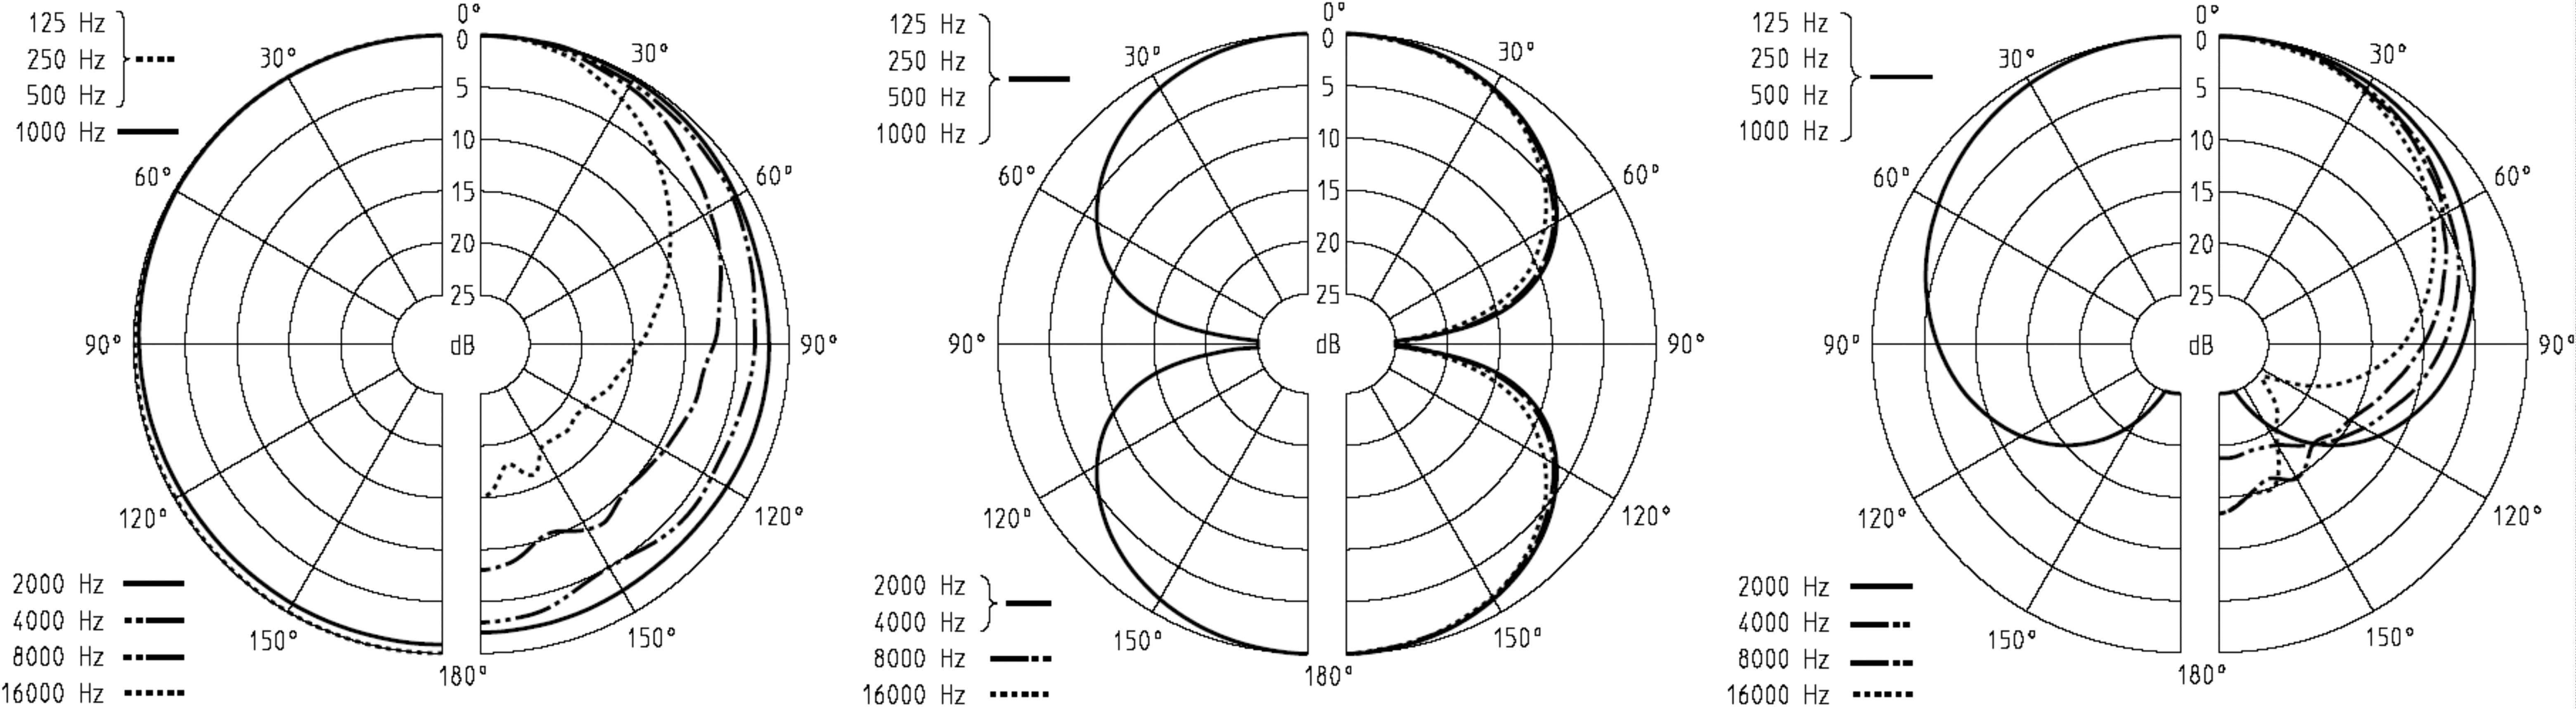
\includegraphics[width=1.0\textwidth]{bilder/3x_richtchars}
\caption[Richtcharakteristiken von Kleinmembran-Studiomikrofonen]{Richtcharakteristiken von Kleinmembran-Studiomikrofonen. V.l.n.r.: Kugel, Acht, Niere. Die Bildbreite ist hier skaliert auf die volle Breite des Satzspiegels.}\label{b_richtch}
% bei langen Bildunterschriften kann der optionale Parameter des caption-Befehls so wie hier für die Kurzfassung im Abbildungsverzeichnis genutzt werden  
\end{figure}
%------------- BILD ENDE ---------------

Für Formelsatz stellt \LaTeX\ die nummerierte Umgebung equation und die nicht-nummerierte Umgebung displaymath zur Verfügung. Mit label und ref kann dann im Text Bezug auf die Gleichungen genommen werden (Gleichung \ref{gl_fourier}). 

\begin{equation}\label{gl_fourier}
S(f) = \int_{-\infty}^{\infty} s(t)e^{-j 2 \pi f t}dt
\end{equation}

Mathematik im Zeilenmodus sieht so aus $f_0 = \frac{1}{2\pi} \sqrt{\frac{s}{m}}$, während dieselbe Gleichung als abgesetzte Formel -- hier mit der displaymath-Umgebung -- so aussieht: 

\begin{displaymath}
f_0 = \frac{1}{2\pi} \sqrt{\frac{s}{m}} 
\end{displaymath}

Für mehrzeilige Herleitungen oder Berechnungen benutzt man in \LaTeX\ die Umgebung eqnarray.

Einheiten innerhalb von Formeln werden -- wie auch Text -- grundsätzlich steil (nicht-kursiv) gesetzt. Innerhalb der mathematischen Umgebung nimmt man dafür eine mbox (make box); die Abstände werden mit Komma, Semikolon oder quad eingestellt:

\begin{displaymath}
f_0 = \frac{1}{2\pi} \sqrt{\frac{s}{m}} \quad \mbox{[Hz]}
% \, kleiner Abstand \; mittlerer Abstand \quad großer Abstand
\end{displaymath}

Gleiches gilt für Funktionsnamen (sin, cos, arctan, log, ...). Für die meisten Funktionsnamen gibt es aber zur Vereinfachung entsprechende Befehle, sodass man nicht immer die mbox braucht.


\section{Unterkapitel mit zwei Zitaten}

Das wörtliche Zitat wird durch Kursivschrift und Anführungszeichen kenntlich gemacht, und natürlich kommt ein Quellenverweis dazu:

% \emph = Texthervorhebung durch Schriftumschaltung (emphasize), \medskip: vertikaler Abstand (\smallskip, \bigskip)
\medskip
\emph{\glqq Ebenso wie die Sinne sind in der Klanggestalt die geistig-ideellen Bereiche mit den physisch-materiellen verbunden, d.h. die sängerische Intention muss sich den Prinzipien der Klangwahrnehmung unterordnen.\grqq} \citep[111]{sowodniok}.
\medskip

Alternativ kann man ein Zitat auch in den laufenden Text einflechten, denn wie schon Sowodniok bemerkte, muss sich 
\emph{\glqq die sängerische Intention [...] den Prinzipien der Klangwahrnehmung unterordnen\grqq} \citep[111]{sowodniok}. 
Die Quellenverweise werden weiter unten erklärt.


\chapter{Ein anderes Kapitel}

\section{Unterkapitel mit Fußnote, Aufzählungen und Tabellen}\label{sec_fussnot}

Fußnoten sollte man sparsam und bewusst verwenden, erklärende Zusätze und Quellenverweise möglichst in den Text integrieren. Damit bleiben Fußnoten v.A. reserviert für wenige Ergänzungen, die den Lesefluss stören würden, aber nicht weggelassen werden sollen\footnote{Und so sieht die Fußnote dann aus}.

Für Aufzählungen stellt \LaTeX\ die beiden Umgebungen itemize und enumerate zur Verfügung. So sieht eine itemize-Aufzählung aus:

\begin{itemize}\setlength{\itemsep}{0ex} % itemsep ist der Abstand zwischen den Punkten der Aufzählung
\item erster Punkt
\item zweiter Punkt
\end{itemize}

Und das ist eine enumerate-Aufzählung:

\begin{enumerate}\setlength{\itemsep}{0ex}
\item erster Punkt
\item zweiter Punkt
\end{enumerate}

Aufzählungen können auch verschachtelt werden. Als Beispiel dient hier eine enumerate-Umgebung innerhalb einer enumerate-Umgebung:

\begin{enumerate}\setlength{\itemsep}{0ex}
\item erster Punkt
\item 
	\begin{enumerate}\setlength{\itemsep}{-0.5ex}
	\item erster Unterpunkt im zweiten Punkt
	\item zweiter Unterpunkt im zweiten Punkt
	\item dritter Unterpunkt im zweiten Punkt
	\end{enumerate}
\item dritter Punkt
\end{enumerate}

Als nächstes folgt ein Beispiel für eine einfache Tabelle. Wie auch die Bilder müssen die Tabellen stets Unterschrift und Nummer und zwingend einen Verweis im Text haben. In \LaTeX\ wird das wie bei den Abbildungen durch den caption-Befehl und das Befehlspaar label und ref gelöst (Tabelle \ref{t_buli}). Für ein modernes Tabellenlayout wird das \LaTeX-booktabs-Paket benutzt (siehe dazu die Kommentare im Quelltext). Die mittlere Spalte ist hier auf feste Breite (6 cm) gesetzt, damit bei viel Text ein automatischer Umbruch erfolgen kann.

%----------- TABELLE START -------------
\begin{table}[htp] 
\centering
\begin{tabular}{r|p{6cm}|c|c}  % Spalten nach Ausrichtung: l, c, r, p{breite}, mit zwei vertikalen Spaltentrennern
%bitte nicht das kleine L "l" und den Vertikalstrich "|" verwechseln!!! :)
% kleines L steht für eine linksbündige Spalte, Vertikalstrich erzeugt eine Trennlinie zwischen zwei Spalten
\toprule
\multicolumn{4}{c}{\large\bfseries Erste Bundesliga, Spielzeit 2011/2012}\\ \midrule
Platz & Verein & TD & Punkte\\ \midrule
1 & Borussia Dortmund & +20 & 29\\ \midrule
2 & Borussia Münchengladbach & +14 & 29\\ \midrule
3 & FC Bayern München & +26 & 28 \\ \midrule
10 & Hertha BSC Berlin (Ballsportclub), Verein aus der Hauptstadt & $-$1 & 18\\
\bottomrule
\end{tabular}
\caption{Bundesligatabelle vom 14. Spieltag}\label{t_buli}
\end{table}
%--------- TABELLE ENDE ---------------

Tabelle \ref{t_buli2} zeigt eine Variante die ein kompakteres und eleganteres Ergebnis liefert, ohne vertikale Striche, dafür mit eingefärbten Zeilen.

%----------- TABELLE START -------------
\begin{table}[htp] 
\rowcolors{1}{}{lgray} % bei jeder Zeile die Farbe wechseln, abwechselnd nix und hellgrau
\centering
\begin{tabular}{rlcc}  % Spalten nach Ausrichtung: l, c, r, p{breite} 
\toprule
\multicolumn{4}{c}{\large\sffamily Erste Bundesliga, Spielzeit 2011/2012}\\ \midrule
1 & Borussia Dortmund & +20 & 29\\ 
2 & Borussia Münchengladbach & +14 & 29\\
3 & FC Bayern München & +26 & 28\\
10 & Hertha BSC Berlin & $-$1 & 18 \\ \bottomrule
\end{tabular}
\caption{Noch eine Bundesligatabelle vom 14. Spieltag}\label{t_buli2}
\end{table}
%--------- TABELLE ENDE ---------------



\section{Unterkapitel mit drei exemplarischen Quellenverweisen}

Quellenverweise werden mit Autorennamen und Jahr in runden Klammern gesetzt. Dazu wird hier das \LaTeX-natbib-Paket genutzt; der citep-Befehl erzeugt die Quellenangabe auf Basis der Einträge im Literaturverzeichnis \citep{bluray}. Auf gleiche Weise lassen sich auch mehrere Quellen zusammenfassen \citep{dooley_streicher,stephenson}. 

Auf Bücher oder andere umfangreichere Quellen soll mit Seitenangabe verwiesen werden. Dafür stellt der Befehle citep  einen optionalen Parameter zur Verfügung. Und so sieht dann die vollständige Quellenangabe aus \citep[116]{kuttruff}. 

Die Quellen sollen im Literaturverzeichnis alphabetisch sortiert sein.


\subsection{Unter-Unterkapitel zu Hyperlinks und Internetquellen}

Die Beispiele unten im Literaturverzeichnis zeigen exemplarisch, welche Angaben zu den Quellen erforderlich sind (siehe dazu auch die Kommentare im \LaTeX-Quelltext). 

Und noch eine \LaTeX-Spezialität zum Schluss: Durch die Einbindung von url- und hyperref-Paket im header werden die Quellenverweise im PDF-Dokument automatisch mit der jeweiligen Quelle im Literaturverzeichnis verlinkt, und bei Internetquellen werden die URLs anklickbar. Zudem werden die Verzeichnisse (Inhaltsverzeichnis, Abbildungs- und Tabellenverzeichnis) mit den jeweiligen Objekten verlinkt, und es werden Links zwischen jedem \emph{label} und  dazugehörigem \emph{ref} erzeugt, also z.B. zwischen Bildverweis im Text und dem Bild. Die Farben der Links können im header frei eingestellt werden. Im hier vorgeschlagenen Layout sind die URLs und die Quellenverweise Dunkelblau, die anderen Links sind nicht hervorgehoben (Schwarz). 


\chapter{Ergebnisse}

Der thematische Teil schließt mit einer klaren inhaltlichen, auf der Grundidee aufbauenden thematischen Zusammenfassung, insbesondere bezogen auf die in der Arbeit gewonnenen eigenen Erkenntnisse und deren mögliche Auswirkungen auf Forschung und Wissenschaft. 

Ganz am Schluss, nach eventuellen Anhängen, nach Abbildungs- und evtl. ( \- )Ta-\ bellenverzeichnis, und nach dem Literaturverzeichnis, folgt die Eigenst{"a}ndigkeitserkl{"a}rung, die unterschrieben werden muss.


\appendix
\chapter{Material}

\section{Fragebögen, Messprotokolle etc.}
In den Anhängen landen ggf. Listings, Fragebögen, Datenblätter, Messprotokolle, Skizzen zu Versuchsaufbauten und ähnliches Material zur Arbeit. Im \LaTeX-Dokument leitet der Befehl appendix die Anhänge ein.



%--------------------- VERZEICHNISSE ----------------

\listoffigures % Abbildungsverzeichnis erzeugen
\listoftables % Tabellenverzeichnis erzeugen

%--------------------- LITERATURLISTE ---------------
% Die Einträge sollen alphabetisch sortiert sein.

\begin{thebibliography}{}

% Formatierung für Internetquelle
% Grundregel: Name, Vorname (falls vorhanden), VÖ-Jahr (falls vorhanden), Titel in Anführungszeichen, URL, Datum des letzten Aufrufs
% zur Formatierung der URL unbedingt den url-Befehl benutzen!!!
\bibitem[Blu-ray Disc Association(2005)]{bluray} 
Blu-ray Disc Association: 
\emph{White paper Blu-ray Disc Format 2.B Audio Visual Application, Format Specifications for BD-ROM}, 
\url{http://www.blu-raydisc.com/Assets/downloadablefile/2b_bdrom_audiovisualapplication_0305-12955-15269.pdf}, 2005, letzter Zugriff: 1. 10. 2012

% Formatierung für Aufsatz / Paper: Titel in Anführungszeichen, Zeitschriftentitel kursiv
\bibitem[Dooley \& Streicher(1982)]{dooley_streicher} 
Dooley, Wesley L.  \& Streicher, Ronald D.:
\glqq M--S Stereo: A Powerful Technique for Working in Stereo\grqq, 
\emph{Journ. Audio Engineering Society} vol. 30 (10), 1982

% Formatierung für Fachbuch, Diplomarbeit o.Ä.: Titel kursiv
\bibitem[Kuttruff(1991)]{kuttruff}
Kuttruff, Heinrich: 
\emph{Room Acoustics}, 3. Aufl., Elsevier 1991

% Formatierung für Fachbuch mit Herausgeber und mehreren Autoren
\bibitem[Spehr(2009)]{spehr}
Spehr, Georg (Hrsg.): 
\emph{Funktionale Klänge}, transcript 2009

% Formatierung für ein einzelnes Kapitel eines speziellen Autors aus einem Fachbuch mit mehreren Autoren
\bibitem[Sowodniok(2009)]{sowodniok}
Sowodniok, Ulrike: 
\glqq Funktionaler Stimmklang -- Ein Prozess mit Nachhalligkeit\grqq, 
in: Spehr, Georg (Hrsg.): \emph{Funktionale Klänge}, transcript 2009

% Formatierung für Aufsatz / Paper: Titel in Anführungszeichen, Zeitschriftentitel kursiv
\bibitem[Stephenson(1990)]{stephenson}
Stephenson, Uwe: 
\glqq Comparison of the Mirror Image Source Method and the Sound Particle Simulation Method\grqq, 
\emph{Applied Acoustics} vol. 29, 1990


\end{thebibliography}

%--------------------- EIGENSTÄNDIGKEITSERKLÄRUNG ---------------
\clearpage\thispagestyle{empty}
\eigen  % im header definiert
%--------------------------------------- ENDE ------------------------------------
\end{document}
%%%%%%%%%%%%%%%%%%%%%%%%%%%%%%%%%%%%











